\section{Topological sorting}

\subsection{Introduction}

\subsubsection{An introductory problem}
You have a number $n$ of tasks to do, and each task have some dependencies over some other tasks that has to be done before.

If I give you these tasks and the list of their dependencies, can you give me the order in which I have to do the tasks?

\begin{center}
  \begin{tabular}{|l|l|}
  \hline
  \textbf{Task} & \textbf{Dependencies}\\
  \hline
  0 & 1,2,3\\
  1 & 2,4\\
  2 & 4\\
  3 & 1,2\\
  4 & -\\
  5 & 1\\
  \hline
  \end{tabular}
\end{center}

This can be viewed as a directed\footnote{In this problem, it is also acyclic. Why?} graph:

\begin{center}
  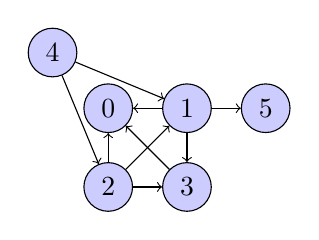
\begin{tikzpicture}[->,nodes={draw, fill=blue!20, circle},row sep=0.3cm,column sep=0.5cm]
    \node (4) {4};
    \node (0) [below right of=4] {0};

    \node (1) [right of=0] {1};
    \node (2) [below of=0] {2};
    \node (3) [right of=2] {3};
    \node (5) [right of=1] {5};

    \draw (1) -> (0);
    \draw (2) -> (0);
    \draw (3) -> (0);
    \draw (2) -> (1);
    \draw (4) -> (1);
    \draw (4) -> (2);
    \draw (1) -> (3);
    \draw (2) -> (3);
    \draw (1) -> (5);
  \end{tikzpicture}
\end{center}

The solution can be derived from a reordering of the vertices:
\begin{center}
  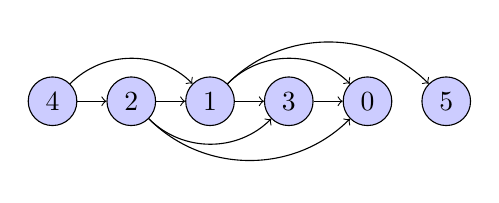
\begin{tikzpicture}[->,nodes={draw, fill=blue!20, circle},row sep=0.3cm,column sep=0.5cm]
    \node (4) {4};
    \node (2) [right of=4] {2};
    \node (1) [right of=2] {1};
    \node (3) [right of=1] {3};
    \node (0) [right of=3] {0};
    \node (5) [right of=0] {5};

    \draw [->] (1) to [bend left=45] (0);
    \draw [->] (2) to [bend right=45] (0);
    \draw (3) -> (0);
    \draw (2) -> (1);
    \draw [->] (4) to [bend left=45] (1);
    \draw (4) -> (2);
    \draw (1) -> (3);
    \draw [->] (2) to [bend right=45] (3);
    \draw [->] (1) to [bend left=45] (5);
  \end{tikzpicture}
\end{center}
\subsubsection{Definition}
A \textbf{topological sort} (sometimes called \textit{toposort}) is an ordering of the vertices of a directed graph, such that, if there is an edge linking vertex $u$ to vertex $v$, we have that $u$ comes before $v$ in the ordering.

\subsubsection{Properties}
\begin{itemize}
\item A topological sort exists for a given graph if and only if there is no directed cycles $==$ if it is a Directed Acyclic Graph (DAG)
\item Every DAG has a valid topological sort;
\item A given DAG may have more than one toposort (for example, our earlier examples accepts three toposorts);
\item If there is a path linking vertices $u$ and $v$, you have that $u$ comes before $v$ in the toposort.
\end{itemize}


\subsection{Algorithm}
The topological sort is in fact the inverse order followed by the DFS \textbf{when "closing" the vertices}.

\begin{lstlisting}[label=code-dfs,caption=DFS algorithm, language=Java, tabsize=2, breaklines=true, numbers=left]
int UNVISITED = 0, OPEN = 1, CLOSED = 2;

void dfsVisit(LinkedList<Integer>[] adj_list, int node, int[] labels)
{
	labels[node] = OPEN;
	for(int new_node : adj_list[node])
		if(labels[new_node] == UNVISITED)
			dfsVisit(adj_list, new_node, labels);
	labels[node] = CLOSED;
}

void dfs(LinkedList<Integer>[] adj_list)
{
	int[] labels = new int[adj_list.length];
	Arrays.fill(labels, UNVISITED);
	for(int node = 0; node < adj_list.length; node++)
		if(labels[node] == UNVISITED)
			dfsVisit(adj_list, node, labels);
}
\end{lstlisting}

When a node $u$ is marked as \texttt{CLOSED}, you have that all nodes to which there is a path from $u$ have already been closed; that means that they lies \textbf{after} $u$ in the toposort.

When then only have to remember the order in which the nodes are closed, and reverse it. We do that using a stack:

\begin{lstlisting}[label=code-toposort,caption=Toposort algorithm, language=Java, tabsize=2, breaklines=true, numbers=left]
int UNVISITED = 0, OPEN = 1, CLOSED = 2;

void dfsVisit(LinkedList<Integer>[] adj_list, int node, int[] labels, Stack<Integer> stack)
{
	labels[node] = OPEN;
	for(int new_node : adj_list[node])
		if(labels[new_node] == UNVISITED)
			dfsVisit(adj_list, new_node, labels, stack);
	labels[node] = CLOSED;
    stack.push(node);
}

Stack<Integer> toposort(LinkedList<Integer>[] adj_list)
{
	int[] labels = new int[adj_list.length];
    Stack<Integer> stack = new Stack<Integer>();
    
	Arrays.fill(labels, UNVISITED);
	for(int node = 0; node < adj_list.length; node++)
		if(labels[node] == UNVISITED)
			dfsVisit(adj_list, node, labels, stack);
    return stack;
}
\end{lstlisting}

\subsection{Exercises}
\begin{enumerate}
\item Do the problem 200 from UVA: \url{http://uva.onlinejudge.org/index.php?option=com_onlinejudge&Itemid=8&page=show_problem&category=24&problem=136}
\item Bonus: do the problem 872 from UVA: \url{http://uva.onlinejudge.org/external/8/872.html}
\end{enumerate}